\chapter{Acids, Bases and pH}\label{ch:g9:acids-bases-ph}

On a kitchen shelf stand a lemon, a bottle of vinegar, a bar of soap and
a box of baking soda; under the sink, a bottle of drain cleaner with a
black-and-red warning label. Some of these taste sour, some feel slippery,
some can burn the skin. One single scale, numbered from 0 to 14, sorts
them all --- and the same scale is used for swimming pools, garden soil,
the blood and the oceans.

\begin{recall}
\omterm{def:g9:ions:ion}{Ions} are \omterm{def:g7:atoms-and-molecules:atom}{atoms} or groups of \omterm{def:g7:atoms-and-molecules:atom}{atoms} carrying a charge; a \omterm{def:g9:ions:ion}{cation} such as
\ce{Na+} is positive, an \omterm{def:g9:ions:ion}{anion} such as \ce{Cl-} or \ce{OH-} negative.
Ionic solutions contain \omterm{def:g9:ions:ion}{ions} marked (aq), which move freely
(\cref{ch:g9:ions}).
\end{recall}

\begin{omfigure}
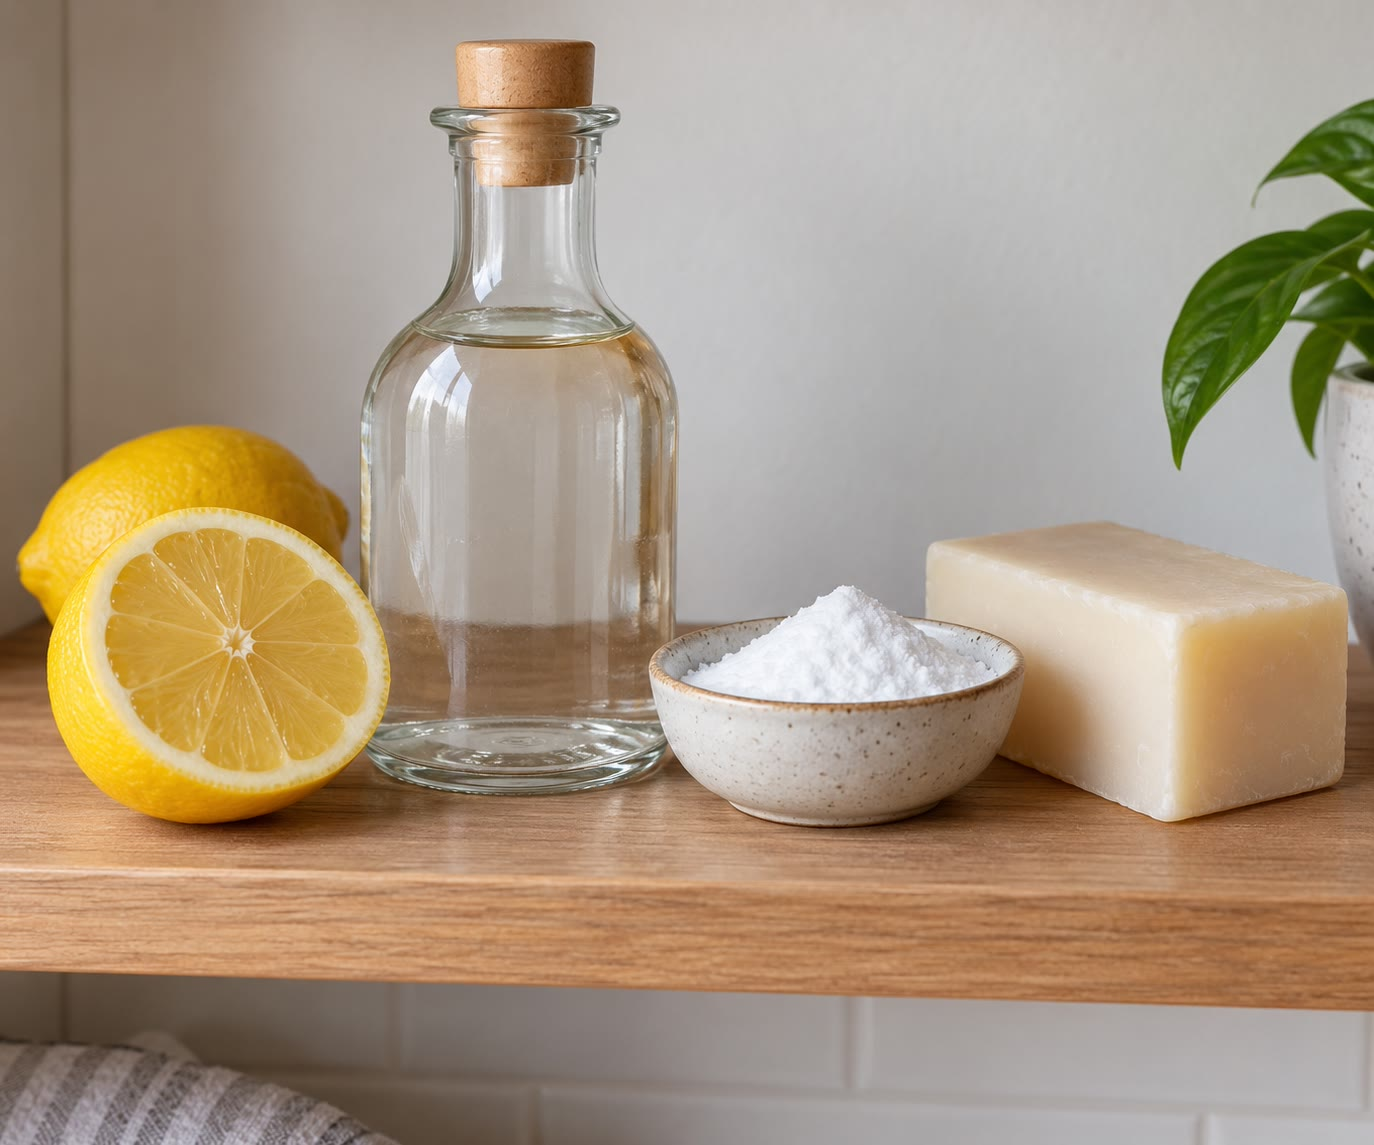
\includegraphics[width=0.55\linewidth]{images/book1/ai/g9-kitchen-shelf.jpg}

{\small Lemon, vinegar, soap and baking soda: acids and bases in the
kitchen.}
\end{omfigure}

\section{Acidic, basic and neutral solutions}

\begin{definition}[Acidic, basic and neutral solutions]\label{def:g9:acids-bases-ph:acidic}
Every \omterm{def:g6:solutions-and-solubility:solute}{aqueous solution} contains hydrogen \omterm{def:g9:ions:ion}{ions} \ce{H+(aq)} and hydroxide
\omterm{def:g9:ions:ion}{ions} \ce{OH-(aq)}. A solution is an \emph{acidic solution}\index{acidic solution}
when it contains more \ce{H+} \omterm{def:g9:ions:ion}{ions} than \ce{OH-} \omterm{def:g9:ions:ion}{ions}, a
\emph{basic solution}\index{basic solution} when it contains more
\ce{OH-} \omterm{def:g9:ions:ion}{ions} than \ce{H+} \omterm{def:g9:ions:ion}{ions}, and a \emph{neutral
solution}\index{neutral solution} when it contains as many of each.
\end{definition}

\begin{example}[Three solutions]\label{ex:g9:acids-bases-ph:three}
Hydrochloric acid is an \omterm{def:g9:acids-bases-ph:acidic}{acidic solution}: it holds \ce{H+(aq)} and
\ce{Cl-(aq)} \omterm{def:g9:ions:ion}{ions}, with very few \ce{OH-}. A sodium hydroxide solution
is basic: \ce{Na+(aq)} and \ce{OH-(aq)}, with very few \ce{H+}. Pure
water and salt water are neutral.
\end{example}

\section{The pH scale}

\begin{definition}[pH]\label{def:g9:acids-bases-ph:ph}
The \emph{pH}\index{pH} of an \omterm{def:g6:solutions-and-solubility:solute}{aqueous solution} is a number, usually
between 0 and 14, that tells how acidic or basic it is: at
\qty{25}{\celsius}, a \omterm{def:g9:acids-bases-ph:acidic}{neutral solution} has pH 7, an \omterm{def:g9:acids-bases-ph:acidic}{acidic solution} a pH
below 7, a \omterm{def:g9:acids-bases-ph:acidic}{basic solution} a pH above 7. The more \ce{H+} \omterm{def:g9:ions:ion}{ions} a solution
holds, the lower its pH.
\end{definition}

\begin{omfigure}
\begin{tikzpicture}[font=\small, x=0.95cm]
  \foreach \k in {0,...,13} {
    \pgfmathtruncatemacro\rr{2.2*max(0,100-14.3*\k)+30}
    \pgfmathtruncatemacro\gg{1.8*(\k<7 ? 30+10*\k : 100-8*(\k-7))+40}
    \pgfmathtruncatemacro\bb{2.2*max(0,14.3*(\k-6))+30}
    \definecolor{phc}{RGB}{\rr,\gg,\bb}
    \fill[phc] (\k,0) rectangle ++(1,0.6);
  }
  \foreach \k in {0,...,14} \node[anchor=north, font=\footnotesize] at (\k,-0.02) {\k};
  \draw[black!60] (0,0) rectangle (14,0.6);
  \node[anchor=south] at (3.5,0.65) {acidic};
  \node[anchor=south] at (7,0.65) {neutral};
  \node[anchor=south] at (10.5,0.65) {basic};
  % ledger: ph:HCl-1M, ph:gastric, ph:lime, ph:wine, ph:coffee, ph:pure-water, ph:seawater, ph:milk-magnesia, ph:ammonia, ph:NaOH-1M
  \foreach \x/\lab/\lev/\anc in {0/{hydrochloric\\ acid (1 M)}/1/north, 1.5/{gastric\\ juices}/3/north east,
      2/{lime\\ juice}/2/north west, 3.5/{wine}/1/north, 5/{coffee}/2/north, 7/{pure\\ water}/3/north,
      8.1/{sea\\ water}/1/north, 10.5/{milk of\\ magnesia}/3/north, 12/{household\\ ammonia}/1/north,
      14/{sodium hydroxide\\ (1 M)}/2/north east} {
    \draw[black!55] (\x,-0.45) -- (\x,-0.45-0.8*\lev);
    \node[anchor=\anc, font=\footnotesize, align=center, inner sep=2pt] at (\x,-0.45-0.8*\lev) {\lab};
  }
\end{tikzpicture}

{\small The \omterm{def:g9:acids-bases-ph:ph}{pH} scale, with the \omterm{def:g9:acids-bases-ph:ph}{pH} of some common solutions.}
\end{omfigure}

\begin{definition}[pH paper and pH meter]\label{def:g9:acids-bases-ph:ph-paper}
\emph{pH paper}\index{pH paper} is a strip of paper soaked in a \omterm{def:g6:pure-substances-and-mixtures:mixture}{mixture}
of dyes that takes a different colour at each \omterm{def:g9:acids-bases-ph:ph}{pH}; a drop of the solution
is put on it and the colour is compared with a chart printed on the box.
A \emph{pH meter}\index{pH meter} measures the \omterm{def:g9:acids-bases-ph:ph}{pH} with a glass probe
dipped in the solution and shows it as a number, to one or two decimal
places.
\end{definition}

\begin{method}[Measuring a pH with pH paper]\label{met:g9:acids-bases-ph:paper}
\begin{enumerate}
  \item Put a short strip of \omterm{def:g9:acids-bases-ph:ph-paper}{pH paper} on a clean, dry dish.
  \item With a clean glass rod, touch the strip with a drop of the
        solution (never dip the strip in the bottle).
  \item Compare the colour at once with the chart, and read the \omterm{def:g9:acids-bases-ph:ph}{pH},
        usually to the nearest whole number.
\end{enumerate}
\end{method}

\begin{omfigure}
\begin{tikzpicture}[font=\small, scale=1.2]
  \pic[transform shape] at (0,0) {stirrer};
  \pic[transform shape] at (0,0.05) {beaker={0.55}{omWater!80}};
  \pic[transform shape] at (0.25,0.35) {probe};
  \pic[transform shape] at (2.6,3.4) {meter={pH}};
  \draw[black!70, line width=0.6pt] (0.25,3.45) .. controls (0.3,4.3) and (2.2,4.4)
    .. (2.2,2.95);
  \draw[<-, omProp, thick] (0.4,1.0) -- (2.0,1.3) node[right, text=black] {glass probe};
  \draw[<-, omProp, thick] (3.35,3.4) -- (4.0,3.4) node[right, text=black] {pH meter};
  \draw[<-, omProp, thick] (-0.6,0.6) -- (-1.6,0.9) node[left, text=black] {solution};
\end{tikzpicture}

{\small Measuring a \omterm{def:g9:acids-bases-ph:ph}{pH} with a \omterm{def:g9:acids-bases-ph:ph-paper}{pH meter}: the glass probe dips in the
solution, which is gently stirred.}
\end{omfigure}

\section{Diluting an acid}

\begin{proposition}[Diluting brings the pH closer to 7]\label{prop:g9:acids-bases-ph:dilution}
Adding water to an \omterm{def:g9:acids-bases-ph:acidic}{acidic solution} spreads its \ce{H+} \omterm{def:g9:ions:ion}{ions} through a
larger volume: the \omterm{def:g9:acids-bases-ph:ph}{pH} goes up, towards 7, but never beyond. For an acid
such as hydrochloric acid, diluting ten times raises the \omterm{def:g9:acids-bases-ph:ph}{pH} by about one
unit: one volume of acid at \omterm{def:g9:acids-bases-ph:ph}{pH} 2 plus nine volumes of water gives a
solution at \omterm{def:g9:acids-bases-ph:ph}{pH} 3. Diluting a \omterm{def:g9:acids-bases-ph:acidic}{basic solution} likewise lowers its \omterm{def:g9:acids-bases-ph:ph}{pH}
towards 7.
\end{proposition}

\begin{omfigure}
\begin{tikzpicture}[font=\small, scale=1.05]
  \foreach \k/\ph/\cc in {0/2/red!38!omWater,1/3/red!24!omWater,2/4/red!12!omWater} {
    \pic[transform shape] at (\k*4.4,0) {beaker={0.55}{\cc}};
    \node[anchor=north, align=center] at (\k*4.4,-0.15) {pH \ph};
  }
  \foreach \k in {0,1} \draw[->, thick, omProp] (\k*4.4+1.1,1.0) -- (\k*4.4+3.3,1.0)
    node[midway, above, text=black, font=\footnotesize, align=center]
    {10 mL + 90 mL\\ of water};
\end{tikzpicture}

{\small Diluting an acid ten times, then ten times again: the \omterm{def:g9:acids-bases-ph:ph}{pH} goes from
2 to 3 to 4 (each beaker is a tenth of the previous solution topped up
with water).}
\end{omfigure}

\begin{inthelab}[Diluting an acid]
To dilute an acid, the teacher always pours the acid slowly into the
water, never the water into the acid: the mixing gives out heat, and
water poured onto a concentrated acid can boil at once and spit acid
out of the container.
\end{inthelab}

\section{Everyday acids and bases}

\begin{proposition}[Acids and bases around us]\label{prop:g9:acids-bases-ph:everyday}
Acidic: lemon and lime juice, vinegar, wine, fizzy drinks, coffee,
gastric juices in the stomach. Basic: sea water (slightly), baking soda
dissolved in water, soap, milk of magnesia (a remedy for stomach
acidity), household ammonia, bleach, drain cleaner (very strongly).
\end{proposition}

\begin{example}[The pH of the ocean]\label{ex:g9:acids-bases-ph:ocean}
% ledger: ph:seawater, ph:ocean-drop
The average \omterm{def:g9:acids-bases-ph:ph}{pH} of the ocean is about 8.1: slightly basic. Since the
industrial era began, carbon dioxide dissolving from the \omterm{def:g4:air-a-mixture-of-gases:air}{air} has lowered
the \omterm{def:g9:acids-bases-ph:ph}{pH} of surface waters by about 0.1: the oceans are slowly becoming
less basic, which harms shellfish and corals.
\end{example}

\begin{omfigure}
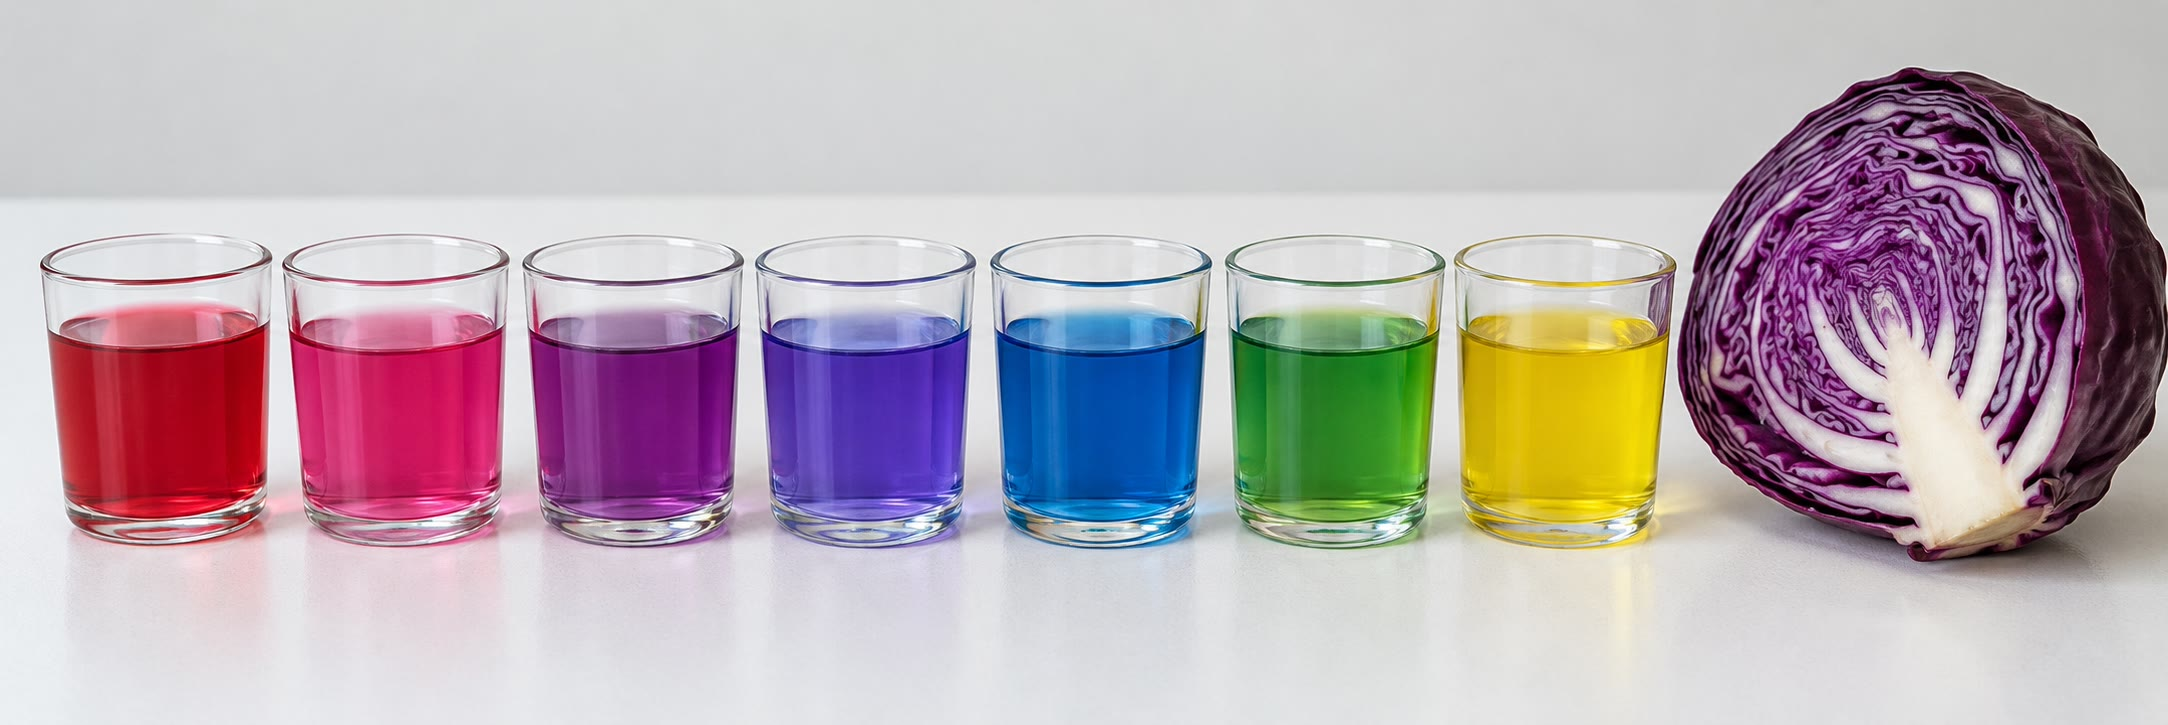
\includegraphics[width=0.55\linewidth]{images/book1/ai/g9-red-cabbage.jpg}

{\small Red cabbage juice, prepared by a teacher, changes colour with the
\omterm{def:g9:acids-bases-ph:ph}{pH}: red in acids, violet near neutral, blue, green then yellow in more
and more \omterm{def:g9:acids-bases-ph:acidic}{basic solutions}.}
\end{omfigure}

\section{Safety with corrosive products}

\begin{safety}{\ghs[0.85cm]{GHS05}\ghs[0.85cm]{GHS07}}
% ledger: ghs:HCl, ghs:NaOH
Concentrated hydrochloric acid and sodium hydroxide (the base of drain
cleaners) carry the corrosion pictogram GHS05: they cause severe burns to
skin and eyes and attack metals. GHS07: irritant. Goggles and gloves; a
splash is rinsed at once with plenty of water.
\end{safety}

\begin{remark}[Never mix cleaning products]\label{rem:g9:acids-bases-ph:mix}
Acidic and basic products react together, sometimes violently, and some
\omterm{def:g6:pure-substances-and-mixtures:mixture}{mixtures} release toxic gases: bleach mixed with an acidic descaler gives
off chlorine. Cleaning products are never mixed.
\end{remark}

\section{Exercises}

\begin{exercise}[$\star$]\label{exo:g9:acids-bases-ph:1}
Acidic, basic or neutral? A solution of \omterm{def:g9:acids-bases-ph:ph}{pH} 3, one of \omterm{def:g9:acids-bases-ph:ph}{pH} 7, one of
\omterm{def:g9:acids-bases-ph:ph}{pH} 11.
\end{exercise}

\begin{exercise}[$\star$]\label{exo:g9:acids-bases-ph:2}
Which \omterm{def:g9:ions:ion}{ions} are more numerous in an \omterm{def:g9:acids-bases-ph:acidic}{acidic solution}? In a basic one?
\end{exercise}

\begin{exercise}[$\star$]\label{exo:g9:acids-bases-ph:3}
Using the \omterm{def:g9:acids-bases-ph:ph}{pH} scale of this chapter, put in order from the most acidic to
the most basic: coffee, sea water, lime juice, household ammonia, pure
water.
\end{exercise}

\begin{exercise}[$\star$]\label{exo:g9:acids-bases-ph:4}
Describe how to measure the \omterm{def:g9:acids-bases-ph:ph}{pH} of a solution with \omterm{def:g9:acids-bases-ph:ph-paper}{pH paper}.
\end{exercise}

\begin{exercise}[$\star\star$]\label{exo:g9:acids-bases-ph:5}
A solution of \omterm{def:g9:acids-bases-ph:ph}{pH} 4 is diluted ten times with water. What is its new \omterm{def:g9:acids-bases-ph:ph}{pH},
about? And if it is diluted a hundred times?
\end{exercise}

\begin{exercise}[$\star\star$]\label{exo:g9:acids-bases-ph:6}
Can an \omterm{def:g9:acids-bases-ph:acidic}{acidic solution} become basic by adding water? Explain.
\end{exercise}

\begin{exercise}[$\star\star$]\label{exo:g9:acids-bases-ph:7}
Why must an acid be poured into water, and not the other way round?
\end{exercise}

\begin{exercise}[$\star\star$]\label{exo:g9:acids-bases-ph:8}
A bottle carries the GHS05 pictogram. What does it mean? Give two
precautions.
\end{exercise}

\begin{exercise}[$\star\star$]\label{exo:g9:acids-bases-ph:9}
How many tenfold dilutions are needed to take an acid from \omterm{def:g9:acids-bases-ph:ph}{pH} 1 to
\omterm{def:g9:acids-bases-ph:ph}{pH} 4? What total dilution is that?
\end{exercise}

\begin{exercise}[$\star\star$]\label{exo:g9:acids-bases-ph:10}
Milk of magnesia is taken for stomach acidity. Using the \omterm{def:g9:acids-bases-ph:ph}{pH} scale,
explain why.
\end{exercise}

\begin{exercise}[$\star\star\star$]\label{exo:g9:acids-bases-ph:11}
The ocean's \omterm{def:g9:acids-bases-ph:ph}{pH} has fallen by about 0.1 since the industrial era. Is the
ocean acidic today? In which direction is it moving, and why?
\end{exercise}

\begin{exercise}[$\star\star\star$]\label{exo:g9:acids-bases-ph:12}
A student measures the \omterm{def:g9:acids-bases-ph:ph}{pH} of the same vinegar with \omterm{def:g9:acids-bases-ph:ph-paper}{pH paper} (3) and with
a \omterm{def:g9:acids-bases-ph:ph-paper}{pH meter} (2.6). Explain why the two results differ and which is more
precise.
\end{exercise}

\section{Problem: The Acid Spill}

\begin{problem}[{Weekend problem --- a litre of acid spilt in a
laboratory sink, and why diluting it is not the answer}]
\label{pb:g9:acids-bases-ph:1}
A bottle containing \qty{1}{L} of dilute hydrochloric acid, of \omterm{def:g9:acids-bases-ph:ph}{pH} 2,
breaks in a laboratory sink. The drain must not receive any solution of
\omterm{def:g9:acids-bases-ph:ph}{pH} below 5. Take the rule of this chapter: for this acid, each tenfold
dilution raises the \omterm{def:g9:acids-bases-ph:ph}{pH} by one unit.

\medskip
\noindent\textbf{Part I --- The acid.}
\begin{enumerate}
  \item Is the solution acidic, neutral or basic? Which \omterm{def:g9:ions:ion}{ions} does it
        contain most?
  \item Which pictogram should the bottle carry, and why?
  \item The teacher measures the \omterm{def:g9:acids-bases-ph:ph}{pH} with a \omterm{def:g9:acids-bases-ph:ph-paper}{pH meter} rather than \omterm{def:g9:acids-bases-ph:ph-paper}{pH paper}.
        Give one advantage.
  \item How many more \ce{H+} \omterm{def:g9:ions:ion}{ions} are there in a litre at \omterm{def:g9:acids-bases-ph:ph}{pH} 2 than in a
        litre at \omterm{def:g9:acids-bases-ph:ph}{pH} 3 of the same acid?
\end{enumerate}

\medskip
\noindent\textbf{Part II --- Diluting.}
\begin{enumerate}[resume]
  \item What volume of solution is obtained by diluting the litre of
        acid ten times? What is its \omterm{def:g9:acids-bases-ph:ph}{pH}?
  \item How many tenfold dilutions are needed to reach \omterm{def:g9:acids-bases-ph:ph}{pH} 5?
  \item What total volume of solution would that make?
  \item Could any amount of water make the solution basic? Explain.
\end{enumerate}

\medskip
\noindent\textbf{Part III --- A better way.}
The teacher instead adds, little by little, a solution of a base until the
\omterm{def:g9:acids-bases-ph:ph-paper}{pH paper} shows 7: the \ce{H+} \omterm{def:g9:ions:ion}{ions} of the acid react with the \ce{OH-}
\omterm{def:g9:ions:ion}{ions} of the base.
\begin{enumerate}[resume]
  \item Write the equation of the reaction between \ce{H+} and \ce{OH-}
        \omterm{def:g9:ions:ion}{ions}.
  \item Why is this better than diluting?
  \item Name an everyday basic product that could be used in a kitchen to
        clean up a small spill of vinegar.
  \item Compute the volume of water that would have to be added to the
        litre of acid to bring it to \omterm{def:g9:acids-bases-ph:ph}{pH} 5.
\end{enumerate}
\end{problem}
